\documentclass[stu,12pt]{apa7}

\usepackage[spanish,mexico]{babel}
\usepackage[style=apa]{biblatex}
\usepackage{geometry}
\usepackage{bookmark}
\usepackage{csquotes}
\usepackage{graphicx}
\usepackage{hyperref}
\usepackage{listings}
\usepackage{xcolor}
\usepackage{import}
\usepackage{xifthen}
\usepackage{pdfpages}
\usepackage{multirow}
\usepackage{transparent}
\usepackage{mathptmx}
\usepackage{amsmath}
\usepackage{amssymb}

\addbibresource{referencias.bib}
\affiliation{Facultad de Inform\'atica, Universidad Aut\'onoma de Quer\'etaro}
\course{G31, Semestre 2, 2014: Desarrollo Humano II}
\professor{Servin González Cecilia}

\hypersetup{
	pdftitle={El impacto que genera la Inteligencia M\'ultiple Intrapersonal y 
	su Conducta durante el Desarrollo Profesional},
	colorlinks=false,
}
\title{El impacto que genera la Inteligencia M\'ultiple Intrapersonal y su
Conducta durante el Desarrollo Profesional}
\shorttitle{Inteligencia M\'ultiple, Conducta en el Desarrollo Personal}
\author{Araiza Cort\'ez Jos\'e Antonio, Baqueiro Lezama Mateo, Bautista Olvera
Marco El\'ias, C\'ardenas Camacho Alexis Emilio, Garc\'ia Mej\'ia Miguel
\'Angel, Gonz\'alez C\'ordoba Bryan Michel, Ju\'arez Ram\'irez Gabriel, Le\'on
L\'opez Michel Christopher, Mac\'ias Fonseca Alejandro, Mata Guerra David, 
Mondrag\'on Fern\'andez Josu\'e Oziel, N\'u\~nez Rodr\'iguez C\'esar de Jes\'us,
Olvera Garc\'ia Marco Antonio, Padr\'on Moya Luis Gabriel, Pichardo Botillo
Blanca Isabel, Pi\~n\'on Garc\'ia Paola, Serv\'in L\'opez Emilio, Ugalde Arias
Alison, Velasco Rom\'an Paola Esmeralda, Zamorano Monzalvo Daniel}
\duedate{16 de mayo de 2024\\
	\begin{center}
	\includegraphics[width=2cm]{./assets/img/escudo-uaq.png}\end{center}
	\begin{center}\includegraphics[width=2cm]
	{./assets/img/escudo-uaq-facultad-informatica.png}
	\end{center}
}

\begin{document}
\maketitle
\tableofcontents
\listoffigures
\listoftables
\section{Introducci\'on}
Aunque la inteligencia intrapersonal se refiere principalmente a la relación de una persona consigo misma, su influencia en las relaciones sociales es significativa y multifacética, esta inteligencia no solo ayuda en la toma de decisiones personales, sino que también contribuye a relaciones sociales más saludables y efectivas. Las personas que se comprenden a sí mismas tienden a ser más conscientes de cómo sus emociones y comportamientos afectas a los demás, por lo que les permite interactuar de manera empática y considerada. 
Por lo que si se reconocen bien las emociones y comportamientos de uno mismo, entonces se podrá identificar los mismos de un individuo de la escuela, hogar o trabajo. 

En este artículo se busca desglosar el como la inteligencia múltiple intrapersonal tiene un impacto significativo en el desarrollo profesional al promover un profundo autoconocimiento, mejorar la toma de decisiones y, facilitar el desarrollo de habilidades.

Se hablará del como se desempeña la inteligencia emocional en el entorno laboral resaltando las capacidades cognitivas que poseen las personas durante su desarrollo profesional, jugando un papel crucial al influir en la toma de decisiones al igual que desenvolverlas en el ámbito laboral.
De igual forma se explicará del autoconocimiento de cada individuo, resaltando y explicando con mayor claridad las propias fortalezas, debilidades, intereses y valores de cada una de las personas, algunas habilidades clave como la autorreflexión, la autogestión y resiliencia, ya que no solo mejoran la capacidad de adaptación antes los obstáculos, retos, cambios, etcétera, sino que también potencian el crecimiento continuo y el bienestar en el entorno laboral. 
También, se tomará en cuenta la introspección, siendo esta vital en el desempeño laboral, ya que este proceso continuo de autoevaluación y ajuste es fundamental para mantener y mejorar el rendimiento profesional.
\section{Planteamiento del Problema}
\section{Planteamiento del Problema}
De primera instancia, se quiso buscar la correlaci\'on de esta inteligencia --
que se denota m\'as como una que trabaja solo con el interior del individuo, sin
embargo, se decidi\'o explorar en esta investigaci\'on el c\'omo es que puede
influir en lo externo. A la vez, con esto se busc\'o relacionar el por qu\'e del
\'exito de individuos catalogados como introvertidos, que normalmente llegan a
desarrollar de una mejor manera esta inteligencia que los individuos
clasificados como extrovertidos
\section{Preguntas de Investigaci\'on}
Para poder tener un mejor esquema de la situaci\'on con la inteligencia
intrapersonal, se decidi\'o seguir un margen de preguntas para poder investigar
su naturaleza
\begin{itemize}
\item ?`Por qu\'e puede influir esta inteligencia en lo externo?
\item ?`C\'omo puede afectar en el trabajo?
\item ?`Se puede desarrollar mejor esta inteligencia para poder tener un mayor
\'exito en el \'area laboral?
\item ?`A qu\'e medios se debe acudir para conocer mejor de manera intr\'inseca
	esta inteligencia?
\item ?`C\'omo se puede evaluar esta inteligencia?
\item ?`Qu\'e representan los resultados al evaluar esta inteligencia?
\item ?`C\'omo puede estar vinculada con la inteligencia emocional?
\end{itemize}

\section{Objetivos}
\subsection{Objetivo General}
Analizar, comprender  y explorar cuál es el papel que toma la inteligencia
intrapersonal en el área del desarrollo profesional, tomando principalmente en
cuenta factores como la importancia que tiene en la conducta, el desempeño y el
éxito laboral conforme el paso del tiempo, así mismo, el impacto que esto genera
en la conexión que existe con las demás gente o equipo de trabajo, considerando
factores esenciales y primordiales.
\subsection{Objetivo Particular}
Analizar y descifrar como la inteligencia intrapersonal juega un papel
importante a la hora de desarrollarse profesionalmente, tomando en cuenta todo
lo positivo así como lo negativo que esto genera, toma de decisiones, control de
estrés, tolerancia , responsabilidad, así como hasta llegar a ser un líder
profesional, explorando e identificando ciertas estrategias y motivaciones para
potenciar esta inteligencia dentro del ámbito, fomentando a desarrollar la
inteligencia intrapersonal para un bien tanto propio como común.

\section{Justificaci\'on}
\documentclass{article}
\begin{document}

\section{Justificación}
Este artículo surge por dos motivos fundamentales. En primer lugar, busca recrear un ambiente laboral en el aula con el objetivo de promover la experiencia del trabajo en equipo. Nos interesa observar cómo el compromiso, la responsabilidad, la gestión del tiempo y el esfuerzo conjunto pueden llevarnos a alcanzar objetivos más ambiciosos que cuando trabajamos de manera individual o en equipos desorganizados.

En segundo lugar, este estudio pretende resaltar la importancia de la introspección en el entorno laboral. A menudo se enfatiza la relevancia de habilidades interpersonales como la comunicación y la expresión, pero rara vez se aborda el valor de la introspección. Este artículo busca demostrar el impacto significativo de la inteligencia intrapersonal en el desarrollo de las''soft skill'' y su influencia positiva en el desempeño laboral.

Al explorar la interacción entre el trabajo en equipo y la introspección, este artículo busca ofrecer una perspectiva más completa sobre cómo las habilidades intrapersonales pueden complementar y potenciar las habilidades interpersonales en un entorno laboral dinámico.

\end{document}


\section{Hip\'otesis}
La Inteligencia Múltiple Intrapersonal, entendida como la habilidad de conocerse a sí mismo, gestionar las emociones y motivarse internamente, tiene una influencia beneficiosa en el desarrollo profesional de las personas. Aquellos individuos con un nivel superior de Inteligencia Interpersonal:
\begin{itemize}
\item Tienen un mayor autoconocimiento y claridad acerca de sus fortalezas, debilidades, intereses y valores, lo que les permite tomar mejores decisiones profesionales alineadas con su perfil.
\item Las emociones manejan mejor, lo que les da estabilidad y les permite enfocarse en sus objetivos profesionales sin dejarse llevar por altibajos emocionales.
\item Se siente motivados internamente, siendo capaces de resistir ante los desafíos y dificultades que surgen en el trayecto laboral.
\item Se desarrollan habilidades como la autorreflexión, la autogestión y la resiliencia, que son fundamentales para el crecimiento y la adaptación en el ámbito laboral.
\end{itemize}

Se espera, por consiguiente, establecer una correlación positiva que los individuos con altos niveles de Inteligencia Intrapersonal demuestren una mayor capacidad para identificar y capitalizar sus fortalezas y debilidades, lo que les permitirá tomar decisiones profesionales más acertadas y alineadas con sus intereses y valores personales. Asimismo, se anticipa que estos individuos serán más efectivos en la gestión de sus emociones, lo que les brindará una mayor estabilidad emocional y les permitirá mantener un desempeño consistente y enfocado en sus metas profesionales a lo largo del tiempo.\\
Además, se plantea que la Inteligencia Intrapersonal favorece la motivación interna y la autoeficacia, aspectos fundamentales para la persistencia y el logro de objetivos profesionales a largo plazo. Se espera que aquellos individuos con una sólida Inteligencia Intrapersonal desarrollen habilidades como la autorreflexión, la autodisciplina y la resiliencia, lo que les permitirá afrontar los desafíos laborales con mayor eficacia y adaptabilidad.\\
En consecuencia, se prevé que en el grupo de estudio, aquellos individuos que exhiban niveles más elevados de Inteligencia Múltiple Intrapersonal experimentarán un mayor éxito, satisfacción y bienestar en sus carreras profesionales en comparación con aquellos con niveles más bajos de esta forma de inteligencia. Esta hipótesis busca explorar y validar la importancia de la Inteligencia Intrapersonal como un factor determinante en el desarrollo y la realización profesional de las personas en el entorno laboral contemporáneo.

\section{Marco Te\'orico}
Todo esto empieza con Howard Garner quien en la década de los 90 presenta la
tesis sobre la existencia de las Inteligencias múltiples, esta teoría nace de
una manera muy peculiar debido que nació directamente de la psicología, pero la
mayoría de los psicólogos les desagradó y otros simplemente las ignoraron, sin
embargo, desde el sector educativo comenzó a poner más atención a esta teoría,
ahí es donde entra Howard Garner para desarrollar totalmente esta idea.\\
Estas inteligencias las define más bien como capacidades que tiene un ser humano
y se van desarrollando a lo largo de su vida. Esta teoría da a conocer que los
conocimientos que adquirimos son de manera intuitiva y no es necesario tener una
brillantez académica para desarrollarla u obtenerla por lo que cada inteligencia
expresa una capacidad que opera de acuerdo a sus propios sistemas, bases o
reglas biológicas, puede haber gente que desarrolle un aspecto mejor que otra de
una manera muy natural, pero eso no significa que la otra persona no sea
inteligente si no que no ha desarrollado la habilidad a comparar pero puede que
esta persona la tenga en otro aspecto o situación. Por esto mismo Gardner da a
conocer que todos tenemos siete inteligencias modulares esto quiere decir que
cada una es autónoma e independiente de las otras, se combinan en el individuo y
el aspecto social, pero entre ellas no se influyen.\\
Las siete inteligencias que present\'o son las siguientes:
\begin{itemize}
\item Lingüístico-verbal.
\item Lógico-matemática.
\item Musical.
\item Espacial.
\item Científico-corporal.
\item Interpersonal.
\item Intrapersonal.
\item Naturalística.
\end{itemize}
Estas son las siete principales, sin embargo en los inicios de los 2000´s,
empezó a investigar dos probables nuevas inteligencias, pero se mantienen
hipotéticos, las cuales son la inteligencia moral que se define como la
habilidad de algunas personas para discernir lo que comúnmente se conoce como el
bien y el mal, y la otra es la inteligencia existencial que esta es un poco más
compleja ya que es la que quiere señalar una sensibilidad por la existencia del
ser humano reflexionando mucho las trascendencia humana.\\
Sin embargo, en este trabajo nos enfocaremos en uno en particular, que es la
inteligencia interpersonal que se define como “la capacidad de entender a los
demás e interactuar eficazmente con ellos. Incluye la sensibilidad a expresiones
faciales, la voz, los gestos y posturas y la habilidad para responder”. En lo
que consiste es el relacionarse y ser empáticos con otras personas, reconocer y
apreciar opiniones, formas de pensar, gustos, etc.; a pesar de etas diferencias
es mantener una relación amable y de buena comunicación siendo respetuoso con
los demás, normalmente se ve este tipo de actitudes en personas que tienen un
oficio que se enfoca mucho al ojo público, como lo son actores, personas de la
farándula, políticos, o gente que represente un grupo social.\\
El enfoque que le daremos a esta inteligencia será dentro del ambiente laboral,
como esta capacidad puede afectar en un ambiente en el cual estas en constante
contacto con personas que tienen distintas personalidades tratando de tener un
gran ambiente. La importancia de tener afinada esta cualidad es mantener un
canal de comunicación efectivo mejorando el trabajo en equipo, capacidad de
resolver conflictos también es muy importante en estos ambientes mostrando
liderazgo y una mentalidad de querer superarse. Aquí entra otro tema que servirá
de mucha importancia, que es la inteligencia emocional quien influye demasiado
en la manera con la que actúas socialmente con las personas.\\
Según Peter Salovey y John Mayer definen la inteligencia emocional como
“la capacidad de controlar y regular los sentimientos de uno mismo y de los
demás y utilizarlos como guía del pensamiento y de la acción”; da a entender que
estos hay que usarlos de manera que ayuden a motivarnos, y controlarlos a pesar
de el estado de nuestro ánimo. Años después Daniel Goleman (2007) dice que “la
inteligencia emocional está relacionada con un conjunto de habilidades que se
basan en la capacidad de reconocer los sentimientos propios y ajenos para que
sirvan de guía al pensamiento y a la acción”; al analizar estas definiciones
coinciden en algunas cosas que son la capacidad de aprender, comprender y
resolver problemas.\\
En el año de 1997 Mayer y Salovey presentaron un modelo donde se dividió a la
inteligencia emocional en 4 habilidades que se presentaran a continuación:
\begin{itemize}
\item Percepción Emocional: Esta identifica y reconoce sentimientos propios y
ajenos, prestar atención a las señales corporales o emocionales que presentan
las personas al interactuar con ellas. 
\item Asimilación emocional: Se tienen en cuenta las emociones de la otra
persona cuando se necesita razonar o solucionar algún problema, priorizando los
procesos cognitivos y centrándose en lo importante.
\item Comprensión Emocional: Es la habilidad de comprender las emociones en
función de relaciones de una manera compleja, además de reconocer posibles
transformaciones de las mismas emociones.
\item Regulación Emocional: Es la capacidad de estar abierto a sentimientos
negativos y positivas, reflexionar y gestionar las emociones de uno mismo y los
demás.
\end{itemize}
Estas cuatro divisiones si los reflexionan se aplicarían de una manera muy
importante en el ambiente laboral, percibiendo las emociones de los compañeros,
así como asimilar los problemas de organización, comunicación que se suelen dar
y manejarlos emocionalmente de una forma correcta y armoniosa, haciendo un clima
laboral mas saludable, casi como una familia. Sin embargo, hay seis puntos que
hay que tomar muy en cuenta para llevarlas a cabo en un buen ambiente laboral
las cuales se presentan a continuación.
\subsection{Prevención de riesgos laborales}
Esta mejora los entornos psicosociales que llevan a una mejora en la empresa,
siendo flexibles en algunas reglas o factores situacionales que se pudieran dar
durante el horario laboral, por ejemplo, el poner horarios flexibles, ofertar
actividades que combatan el estrés en la oficina, autonomía en la organización
del trabajo entre muchas más.
\subsection{Motivación}
Según Oropeza (2014), los individuos necesitan sentirse valorados y que sus
esfuerzos en la empresa sean reconocidos, ya que es una de las maneras por los
que la motivación en éstos aumentará, dado que se sentirán a gusto y realizados.
\subsection{Negociación}
Las emociones tienen un papel muy importante en la negociación, ya que muchos
autores establecen que los negociadores que logren una mayor comprensión de las
experiencias y expresiones emocionales estarán mejor preparados para la
negociación. Así pues, los negociadores con una alta IE conseguirán información
de una forma más rápida, tomarán decisiones más objetivas, mostrarán las
emociones adecuadas e inducirán la emoción deseada en el oponente. (López, 2013)
.
\subsection{Gestión y resolución del conflicto}
Hay conflictos que en cuanto aparecen deben desaparecer, en cambio, en
determinadas circunstancias, es necesario incentivarlo para que el resultado del
equipo tenga una gran calidad. Resolver un conflicto significa reducirlo o
eliminarlo; pero gestionarlo implica diseñar estrategias para incrementar la
efectividad de la organización. (Munduate y Medina, 2015).
\subsection{Estrés}
Es una condición mental y física que puede llegar cuando se presiona con mucha
carga a los empleados o trabajadores de una empresa, pero no es todo negativo ya
que si aparece en una dosis adecuada da como una motivación para asumir y
realizar determinadas tareas.
\subsection{Liderazgo}
El liderazgo es uno de los roles que más trabajo emocional implica, debido a que
tienen que estar en un contacto directo con sus colaboradores. Por tanto, la
capacidad de un líder para llevar a un grupo a conseguir unos objetivos es un
tema que tiene una gran importancia como proceso grupal en una organización.
(López, 2013).

\section{Metodolog\'ia de la Investigaci\'on}
\subsection{Enfoque de la investigación}
Dado que se busca comprender y comprobar la hipótesis previamente establecida,
así como los objetivos trazados, el presente trabajo será elaborado bajo el
planteamiento metodológico del enfoque mixto.
\subsection{Tipo de Estudio Observacional}
Un estudio observacional es un tipo de estudio en el que el investigador no interviene en las
variables de estudio. En otras palabras, el investigador se limita a observar los valores de
las variables estudiadas y hacer mediciones. A continuación, te proporciono más detalles
sobre los estudios observacionales
\subsection{El enfoque mixto}
Los estudios con enfoque mixto representan un 
\begin{quote}
conjunto de procesos sistemáticos , empíricos y críticos de investigación e
implican la recolección y el análisis de datos cuantitativos y cualitativos, así
como su integración y discusión conjunta, para realizar inferencias producto de
toda la información recabada y lograr un mayor entendimiento del fenómeno bajo
estudio \parencite{unitec}
\end{quote}
Este enfoque permite abordar preguntas de investigación desde diferentes
perspectivas y enriquecer los resultados obtenidos.
\subsubsection{Variables de estudio}
\begin{itemize}
\item Variables independientes: inteligencia intrapersonal, medida a través de pruebas estandarizadas que evalúan las diferentes dimensiones intrapersonales.
\item Variables dependientes: Desarrollo profesional, medido mediante indicadores como logros profesionales o satisfacción laboral.
\end{itemize}
\subsection{Encuestas}
Realizamos encuestas con el fin de recopilar información relevante y necesaria para lograr
comprender y comprobar nuestra hipótesis y objetivos establecidos previamente. Las
encuestas se llevaron a cabo en persona. Se realiz\'o una encuesta a un grupo de estudiantes. A continuación, las preguntas que realizamos en las encuestas
\subsubsection{Datos demogr\'aficos}
\begin{itemize}
\item Edad
\item Nivel educativo
\item \'Area de estudio o especialidad
\end{itemize}
\subsubsection{Autoevaluaci\'on de inteligencia intrapersonal}
\begin{itemize}
\item  En una escala del 1 al 5, ¿cómo calificarías tu capacidad para conocerte a ti mismo/a?
\item  ¿Consideras que gestionas eficazmente tus emociones en el ámbito profesional? 
\item  ¿Te consideras una persona motivada internamente en tu carrera profesional? 
\end{itemize}
\subsubsection{Percepci\'on sombre la influencia de la inteligencia
intrapersonal en el desarrollo profesional}
\begin{itemize}
\item ¿Crees que tener un buen autoconocimiento influye en la toma de decisiones profesionales?
\item ¿Cómo crees que la gestión emocional impacta en el desempeño laboral?
\item ¿Consideras que la motivación interna es clave para el éxito en la carrera profesional?
\item ¿Qué habilidades asociadas a la inteligencia intrapersonal crees que son más importantes para el desarrollo profesional? (Por ejemplo: autorreflexión, autodisciplina, resiliencia)
\end{itemize}
\subsubsection{Eperiencias y estrategias personales}
\begin{itemize}
\item ¿Has experimentado situaciones donde la inteligencia intrapersonal haya sido crucial para resolver problemas en el trabajo/estudios?
\item ¿Qué estrategias utilizas para mejorar tu inteligencia intrapersonal en el ámbito laboral?
\end{itemize}
\subsubsection{Opini\'on sobre la importancia de la inteligencia intrapersonal
en el entorno laboral}
\begin{itemize}
\item ¿Crees que la inteligencia intrapersonal debería ser más valorada en el ámbito laboral? 
\item ¿Qué medidas crees que podrían implementarse para fomentar el desarrollo de la inteligencia intrapersonal en el lugar de trabajo?
\end{itemize}

\section{Poblaci\'on y Muestra}
Para la investigación sobre ``El impacto que genera la Inteligencia Múltiple Intrapersonal y su conducta durante el desarrollo profesional'', se tomó como población a los estudiantes de nivel superior (universitarios) que estudian la carrera de Ingeniería Informática en la Universidad Autónoma de Querétaro en el campus Juriquilla. Se eligió esta población debido a que se espera un mayor impacto, dado que el entorno de la carrera y el ámbito profesional se desarrollarán en colaboración con más personas, lo cual potenciará la influencia de la inteligencia múltiple intrapersonal. Como muestra, se seleccionó el grupo 31 de dicha carrera, universidad y campus, ya que es el grupo con mayor interacción entre sus integrantes, generando así un mayor nivel de discusión y comunicación a lo largo de todos los días.

\section{T\'ecnicas e Instrumentos de Investigaci\'on}
Para esta investigación, el uso de técnicas e instrumentos adecuados es importante para la obtención de datos precisos y que sean relevantes. Estos métodos nos permiten explorar, analizar y comprender diferentes contextos de una manera estructurada y sistemática. Entre los diversos instrumentos de investigación que se pueden utilizar, decidimos utilizar las encuestas gracias a su eficacia para recopilar información de grandes grupos de personas en un tiempo relativamente corto. 

Esta encuesta, nos permitió obtener percepciones, opiniones y comportamientos de los participantes respecto a temas específicos. Las preguntas formuladas no sólo recogen información cuantitativa sino también cualitativa, proporcionando una visión integral del tema estudiado. En particular, la encuesta fue dirigida a los estudiantes del grupo 31 de la carrera de Ingeniería en Software. Este grupo específico de encuestados ofrece una perspectiva única sobre cómo los futuros profesionales en el ámbito tecnológico pueden llegar a percibir y gestionar su inteligencia intrapersonal. 

A continuación se presentan las preguntas que formaron parte de la encuesta realizada y por qué de dichas preguntas.

\begin{enumerate}
\item Edad\\
Explicación: La edad puede influir en el nivel de desarrollo de la inteligencia intrapersonal, ya que las experiencias y la madurez suelen aumentar con el tiempo, afectando la autoevaluación y gestión emocional.
\item En una escala del 1 al 5 ?`c\'omo calificar\'ias tu capacidad para conocerte
a ti mismo(a)?\\
Explicación: Esta pregunta ayuda a medir directamente la autoevaluación de la inteligencia intrapersonal, proporcionando una visión del nivel de autoconocimiento del encuestado.
\item ?`Consideras que podr\'ias gestionar eficazmente tus emociones en el \'ambito
profesional?\\
Explicación: La gestión emocional es una componente clave de la inteligencia intrapersonal, y esta pregunta evalúa cómo los encuestados perciben su capacidad para manejar emociones en un contexto profesional.
\item ?`Te consideras una persona motivada internamente en tu carrera profesional?\\
Explicación: La motivación interna es otro aspecto esencial de la inteligencia intrapersonal. Evaluar esto ayuda a entender si los individuos se sienten impulsados por factores internos en su desarrollo profesional.
\item ?`Crees que tener un buen autoconocimiento influye en la toma de decisiones
Explicación: Esta pregunta explora la percepción de los encuestados sobre la relevancia del autoconocimiento en la toma de decisiones, un aspecto crítico del desarrollo profesional.
profesionales?\\
\item ?`C\'omo crees que la gesti\'on emocional impacta en el desempe\~no laboral?\\
Explicación: Evaluar la percepción sobre la gestión emocional permite entender cómo los alumnos creen que sus habilidades intrapersonales podrían afectar su rendimiento en el trabajo.
\item ?`Consideras que la motivaci\'on interna es clave para el \'exito en la carrera profesional?\\
Explicación: Esta pregunta investiga la importancia a la motivación interna en el éxito profesional, una faceta de la inteligencia intrapersonal que puede ser crucial para el desarrollo profesional.
\item ?`Has experimentado situaciones donde la inteligencia intrapersonal haya sido
crucial para resolver problemas en el trabajo/estudios?\\
Explicación: Esta pregunta busca ejemplos prácticos donde la inteligencia intrapersonal ha sido aplicada, proporcionando evidencia real de su importancia y utilidad en situaciones específicas.
\item ?`Crees que la inteligencia intrapersonal deber\'ia ser m\'as valorada en el
\'ambito laboral?\\
Explicación: Esta pregunta aborda la importancia de la inteligencia intrapersonal en el lugar de trabajo, lo cual puede influir en políticas y prácticas dentro de una área laboral.

\subsection{Resultados Crudos}
Ver tablas
\ref{tab:pregunta1},
\ref{pregunta2},
\ref{pregunta3},
\ref{pregunta4},
\ref{pregunta5},
\ref{pregunta7},
\ref{pregunta8} y
\ref{pregunta9}
\begin{table}
	\caption{Pregunta 1\label{tab:pregunta1}}
\begin{tabular}{cc}
\hline
Edad & Cantidad Personas\\
\hline
18 & 10\\
19 & 6\\
20 & 1\\
21 & 1\\
22 & 2\\
23 & 1\\
\hline
\end{tabular}
\end{table}
\begin{table}
	\caption{Pregunta \thetable\label{pregunta2}}
\begin{tabular}{cc}
\hline
Respuestas & Cantidad Personas\\
\hline
1 & 2\\
2 & 3\\
3 & 6\\
4 & 8\\
5 & 2\\
\hline
\end{tabular}
\end{table}
\begin{table}
	\caption{Pregunta \thetable\label{pregunta3}}
\begin{tabular}{cc}
\hline
Respuestas & Cantidad Personas\\
\hline
S\'i & 13\\
No & 8\\
\hline
\end{tabular}
\end{table}
\begin{table}
	\caption{Pregunta \thetable\label{pregunta4}}
\begin{tabular}{cc}
\hline
Respuestas & Cantidad Personas\\
\hline
S\'i & 10\\
No & 11\\
\hline
\end{tabular}
\end{table}

\begin{table}
	\caption{Pregunta \thetable\label{pregunta5}}
\begin{tabular}{cc}
\hline
Respuestas & Cantidad Personas\\
\hline
S\'i & 21\\
No & 0\\
\hline
\end{tabular}
\end{table}
En la pregunta 6, se dieron varias respuestas entre las que más se repiten están
\begin{itemize}
\item Aumenta la productividad diaria. 
\item Mejora la comunicación interna. 
\item Reduce el estrés laboral. 
\item Fomenta un ambiente positivo. 
\item Incrementa la motivación personal.
\end{itemize}
\begin{table}
	\caption{Pregunta 7\label{pregunta7}}
\begin{tabular}{cc}
\hline
Respuestas & Cantidad Personas\\
\hline
S\'i & 21\\
No & 0\\
\hline
\end{tabular}
\end{table}
\begin{table}
	\caption{Pregunta 8\label{pregunta8}}
\begin{tabular}{cc}
\hline
Respuestas & Cantidad Personas\\
\hline
S\'i & 15\\
No & 6\\
\hline
\end{tabular}
\end{table}
\begin{table}
	\caption{Pregunta 9\label{pregunta9}}
\begin{tabular}{cc}
\hline
Respuestas & Cantidad Personas\\
\hline
S\'i & 17\\
No & 4\\
\hline
\end{tabular}
\end{table}
\end{enumerate}

\section{Recopilaci\'on de Datos}
\begin{center}
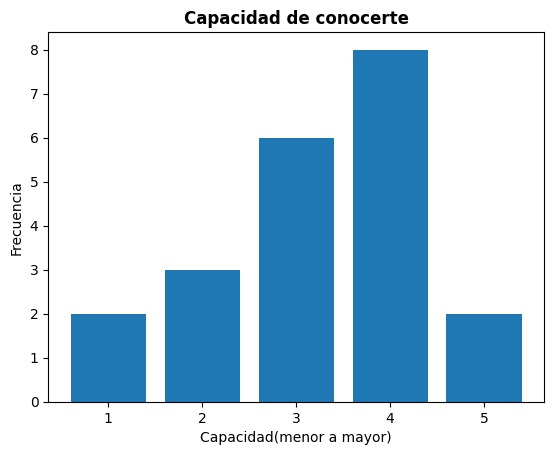
\includegraphics[width=0.8\textwidth]{./assets/img/grafica-1.jpeg}
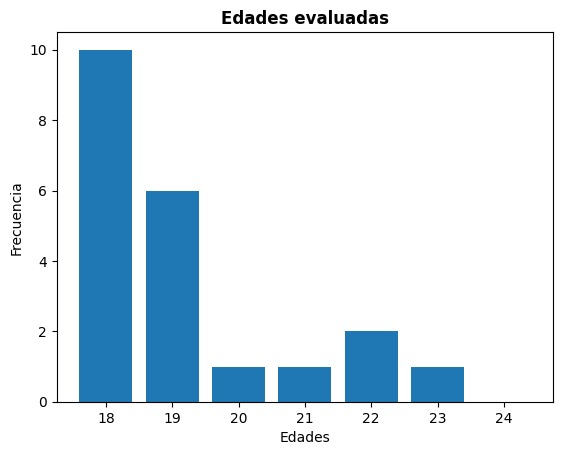
\includegraphics[width=0.8\textwidth]{./assets/img/grafica-2.jpeg}
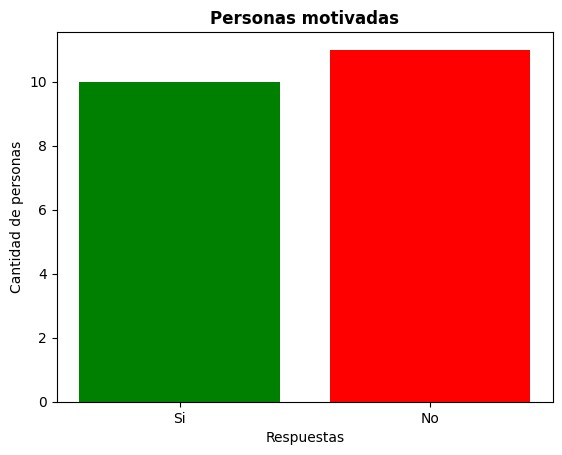
\includegraphics[width=0.8\textwidth]{./assets/img/grafica-3.jpeg}
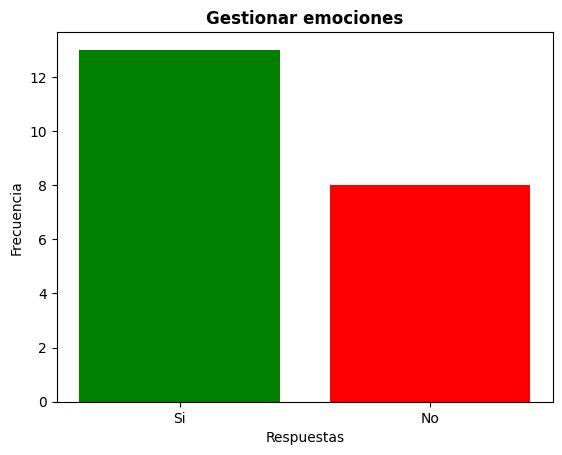
\includegraphics[width=0.8\textwidth]{./assets/img/grafica-7.jpeg}
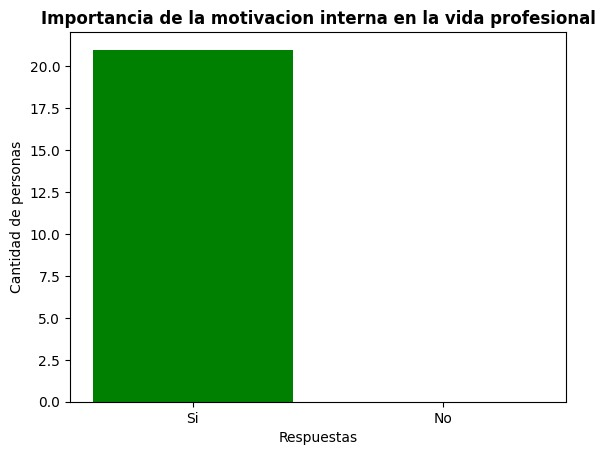
\includegraphics[width=0.8\textwidth]{./assets/img/grafica-5.jpeg}
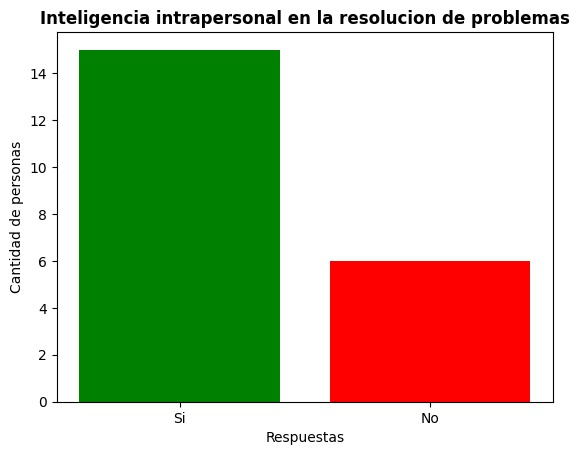
\includegraphics[width=0.8\textwidth]{./assets/img/grafica-7-1.jpeg}
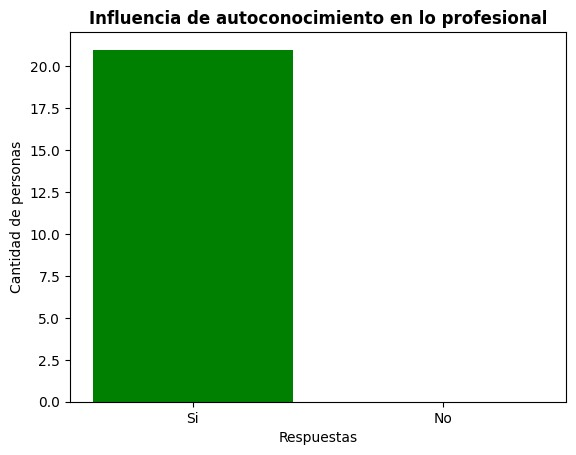
\includegraphics[width=0.8\textwidth]{./assets/img/grafica-8.jpeg}
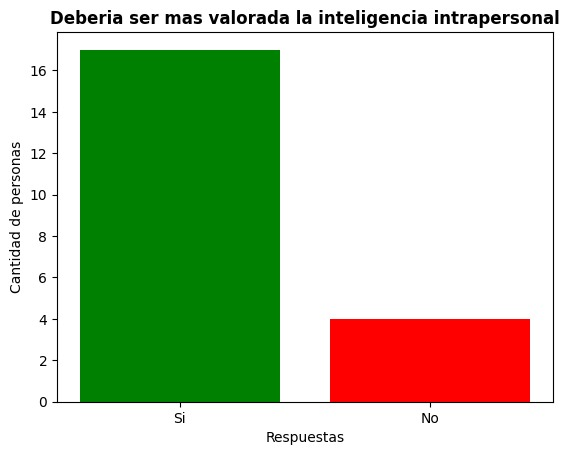
\includegraphics[width=0.8\textwidth]{./assets/img/grafica-9.jpeg}
\end{center}

\section{An\'alisis de Resultados}
El presente trabajo se elaboró bajo el planteamiento de un enfoque metodológico de un enfoque
mixto. Para llevar a cabo esta investigación, se emplearon métodos cualitativos y cuantitativos
realizando un cuestionario basado en 9 preguntas , este cuestionario se les realizó a 21 estudiantes
de segundo semestre de la carrera de ingeniería en software dentro de la Universidad Autónoma de
Querétaro Facultad de informática
Este enfoque permite abordar preguntas de investigación desde diferentes perspectivas y enriquecer
los resultados obtenidos.

Las preguntas de la encuesta se enfocaron en aspectos como:
\begin{itemize}
\item Identificación del autoconocimiento y autorreflexión de los sujetos estudiados.
\item Influencia de la conducta en ámbitos profesionales.
\item Motivación intrínseca y metas profesionales.
\item Gestión y resolución de conflictos.
\item Prevención de riesgos laborales.
\item Percepción, comprensión y asimilación emociona
\end{itemize}
El cuestionario fue profundizado en experiencias más personales en base a algunas percepciones
subjetivas sobre cómo la inteligencia intrapersonal ha influido en su ámbito laboral.
Los resultados mostraron que la mayoría de los estudiantes se consideran con una alta inteligencia
intrapersonal ya que en un ámbito tecnológico pueden llegar a percibir y gestionar su personalidad,
sus capacidades y sus emociones de una manera eficaz

En el cuestionario se incluyeron las siguientes preguntas
\begin{enumerate}
\item Edad
\item En una escala del 1 al 5, ¿cómo calificarías tu capacidad para conocerte a ti mismo/a?
\item ¿Consideras que podrías gestionar eficazmente tus emociones en el ámbito profesional?
\item ¿Te consideras una persona motivada internamente en tu carrera profesional?
\item ¿Crees que tener un buen autoconocimiento influye en la toma de decisiones profesionales?
\item ¿Cómo crees que la gestión emocional impacta en el desempeño laboral?
\item ¿Consideras que la motivación interna es clave para el éxito en la carrera profesional?
\item ¿Has experimentado situaciones donde la inteligencia intrapersonal haya sido crucial para resolver problemas en el trabajo/estudios?
\item ¿Crees que la inteligencia intrapersonal debería ser más valorada en el ámbito laboral?
\end{enumerate}

\subsection{Resultados y Estad\'isticas}
En la pregunta uno se muestran las edades de los encuestados, la edad que predominó con más del
50\% fue la de 10 alumnos con 18 años, 6 alumnos con 19 años, 1 alumno con 20 años, 1 alumno con
21 años, 2 alumnos con 22 años con y 1 alumno con 23 años.\\
Para la pregunta dos hace un análisis en base a una puntuación del 1 (siento la calificación menor)
hasta el 5 (siendo la calificación mayor) y esta refleja que 8 alumnos consideran un 4 como su
capacidad de conocerse a sí mismo, 6 alumnos optan por una puntuación de 3, 3 alumnos con una
puntuación de 2, 2 alumnos con 1 punto y finalmente 2 alumnos con 5 puntos.\\
La pregunta tres se centra en poder saber la eficacia de los alumnos al gestionar sus emociones en el
ámbito laboral, en esta pregunta se pudo analizar que el 61.9 \% (13 alumnos)de los alumnos SI
pueden gestionar con eficacia, por otro lado, el 38.1 \% (8 alumnos) de los alumnos NO se creen
capaces.\\
La pregunta cuatro muestra a los estudiantes que se muestran motivados internamente en tu carrera
profesional, de lo cual el 52.38\% (11 alumnos) de los alumnos NO cuentan con esa motivación,
mientras que el 47.6p2 \% (10 alumnos) SI tiene esa motivación.\\
La pregunta cinco hace referencia al saber de cada alumno por la necesidad del autoconocimiento
de su toma de decisiones profesionales, en este caso se obtuvo un resultado del 100 \% ya que 21
alumnos votaron que SI creen que al tener un buen autoconocimiento influye en la toma de
decisiones profesionales.\\
Dentro de la pregunta seis se quería saber si los alumnos tienen la noción de como la gestión
emocional impacta en el desempeño laboral y se reflejaron varias respuestas, algunas de las más
relevantes y repetitivas fueron:
\begin{itemize}
\item Aumenta la productividad diaria.
\item Mejora la comunicación interna.
\item Reduce el estrés laboral.
\item Fomenta un ambiente positivo.
\item Incrementa la motivación personal.
\end{itemize}
La pregunta siete se realizó con la finalidad de ver la consideración de cada alumno a cerca de la
motivación interna y si la consideran clave para el éxito en la carrera profesional, se obtuvo una
respuesta de un 100 \% por parte de los alumnos, ya que 21 de los 21 alumnos optan que la motivación
interna SI es clave para el éxito en la carrera profesional.\\
Para la pregunta ocho se basa en una pregunta más personal ya que al realizar esta pregunta se tiene
el propósito de saber si los alumnos han experimentado situaciones donde la inteligencia
intrapersonal haya sido crucial para resolver problemas en el trabajo/estudios, y se obtuvo como
resultado que: el 71.43\% (15 alumnos) SI han vivido está experiencia y el 28.57 \% (6 alumnos) NO la
han vivido.\\
En la pregunta nueve se considera el valor individual que le tiene a la inteligencia intrapersonal y si
consideran que se le debería de dar más valor dentro del ámbito laboral. En base a esta pregunta, se
pudo analizar que por mayoría, el 80.95\% (17 alumnos) de los alumnos SI creen que su valor debe
de ser mayor, mientras que el 19.05\% (4 alumnos) dice lo contrario. Como dato relevante,
El 85\% de los encuestados con alta inteligencia intrapersonal reportaron
habilidades superiores en la resolución de conflictos, en contraste con el 40\% de aquellos con baja
inteligencia intrapersonal.
La investigación empleó una técnica principal: encuesta. Las encuestas proporcionaron datos
cuantitativos sobre la población estudiada ya que midieron diversos aspectos de la inteligencia
intrapersonal basándose en un ámbito personal.

\section{Presentación de Resultados}

Por medio del trabajo de investigación se ha indagado y aplicado los conocimientos teóricos de los investigadores, además de las habilidades desarrolladas según los contenidos con respecto a la inteligencia múltiple intrapersonal y su relación con la conducta que genera a lo largo del desarrollo profesional, esto por medio del análisis de su impacto. 

Partimos de una introducción que recopila las ideas principales y contenido del proyecto, se planteó la problemática seleccionada y se generaron preguntas de apoyo para delimitar adecuadamente las ideas, todo esto manteniendo fijos los objetivos deseados y su aplicación, contando con los fundamentos y justificaciones convincentes y objetivos, de forma que se llegó a una hipótesis pertinente, la cual procedió a ser evaluada por un marco teórico bien estructurado y que pudo complementarse más adelante con una metodología que cerrara las ideas y las mantuviera en un enfoque oportuno. 

Por medio de las consideraciones previamente mencionadas, se analizó a una muestra por un instrumento de investigación definido previamente, la cual estaba conformada por los integrantes del grupo. Finalmente cabe destacar que en la investigación se recopila y analiza la información rescatada, pasando por un análisis e implementación con el objetivo principal y los apartados iniciales del proyecto. 

\section{Conclusión}

La realización de la investigación ha representado por parte de los integrantes el dominio de unidades previas, contando con su entendimiento y aplicación para alcanzar el objetivo en común. Pese a las distintas complicaciones que se puedan llegar a presentar, desde la falta de entendimiento hasta problemáticas en la comunicación, la importancia radica en la mejora de nosotros mismos como profesionistas y los cimientos con los que estamos construyendo nuestro futuro.

\begin{appendix}
\section{Im\'agenes del Grupo Trabajando}
\begin{figure}
    \caption{El d\'ia 10 de marzo del 2024 se llev\'o a cabo la decisi\'on sobre el tema del proyecto final y se asignaron los respectivos roles. Grupo 31, 2024.\label{fig:No.1}}
    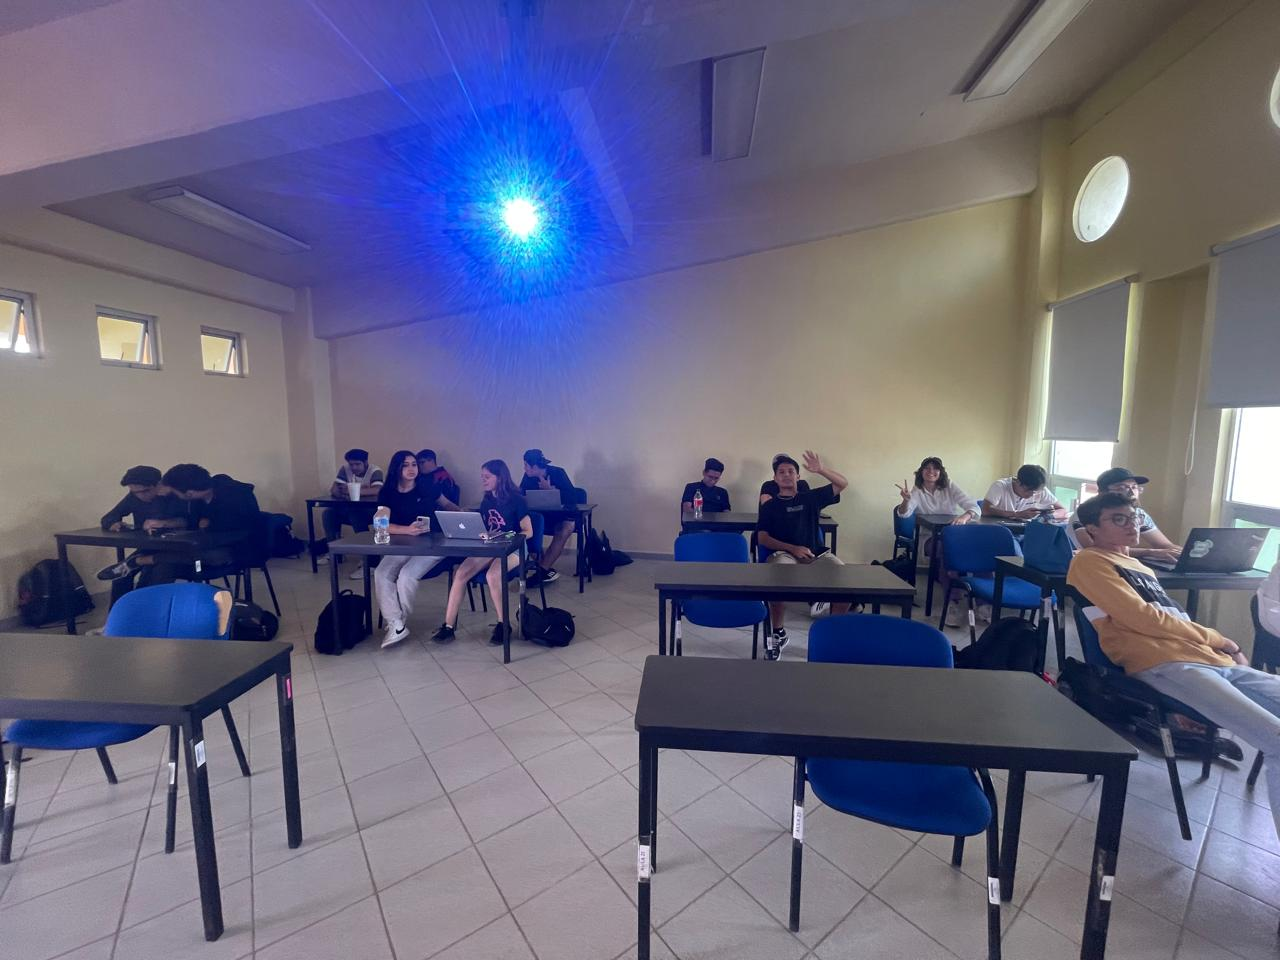
\includegraphics[width=0.7\textwidth]{./assets/img/imagen2DH.jpeg}
\end{figure}

\begin{figure}
    \caption{El d\'ia 21 de marzo del 2024 se realiz\'o una actividad de retroalimentaci\'on sobre el tema ``Inteligencias M\'ultiples''.\label{fig:No.2}}
    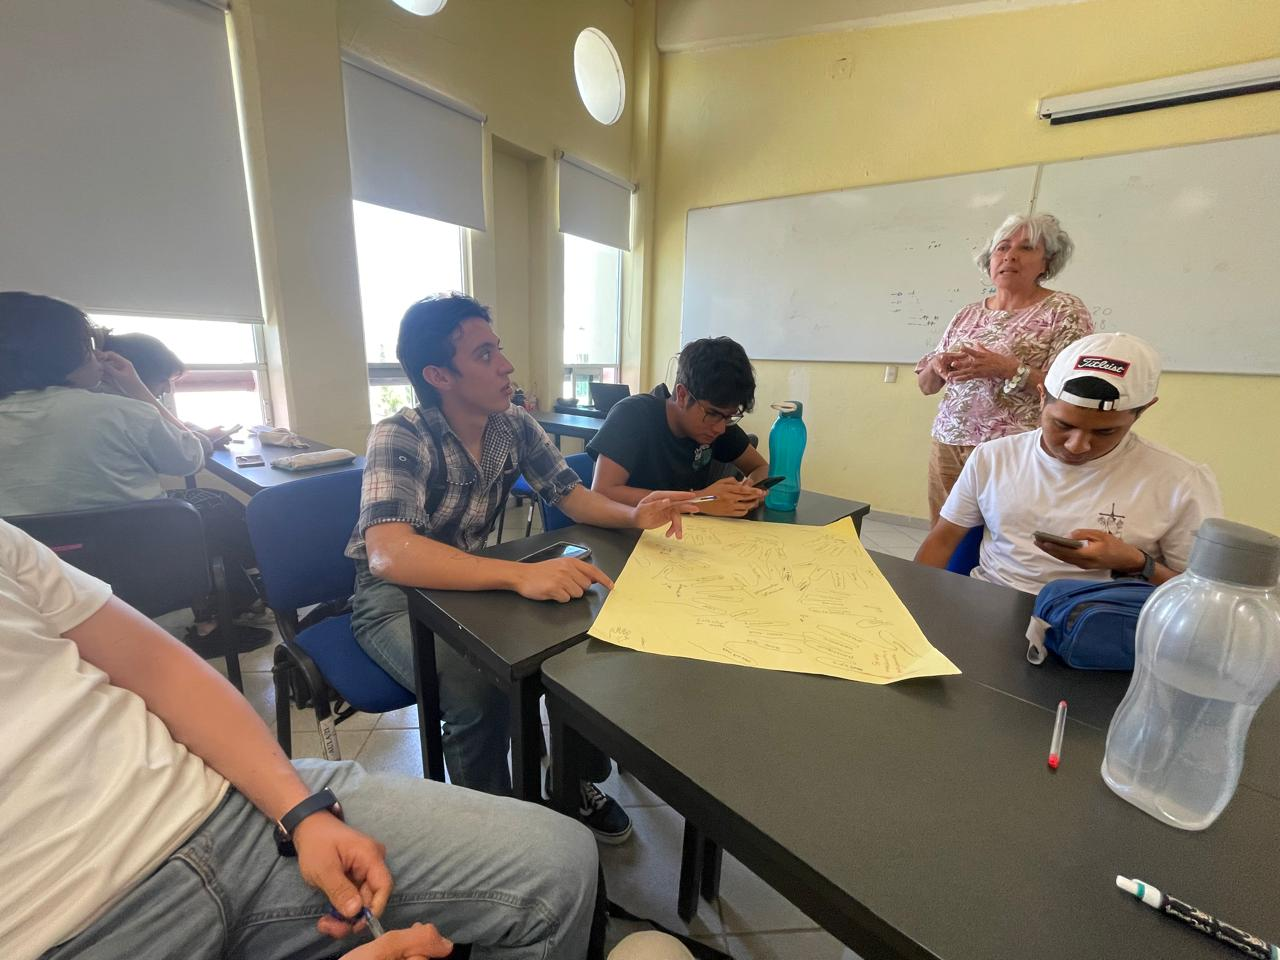
\includegraphics[width=0.7\textwidth]{./assets/img/imagen1DH.jpeg}
\end{figure}

\begin{figure}
    \caption{El d\'ia 2 de Mayo de 2024 se llev\'o a cabo la clase enfocada a la inteligencia emocional en el ámbito laboral. Grupo 31, 2024.\label{fig:No.3}}
    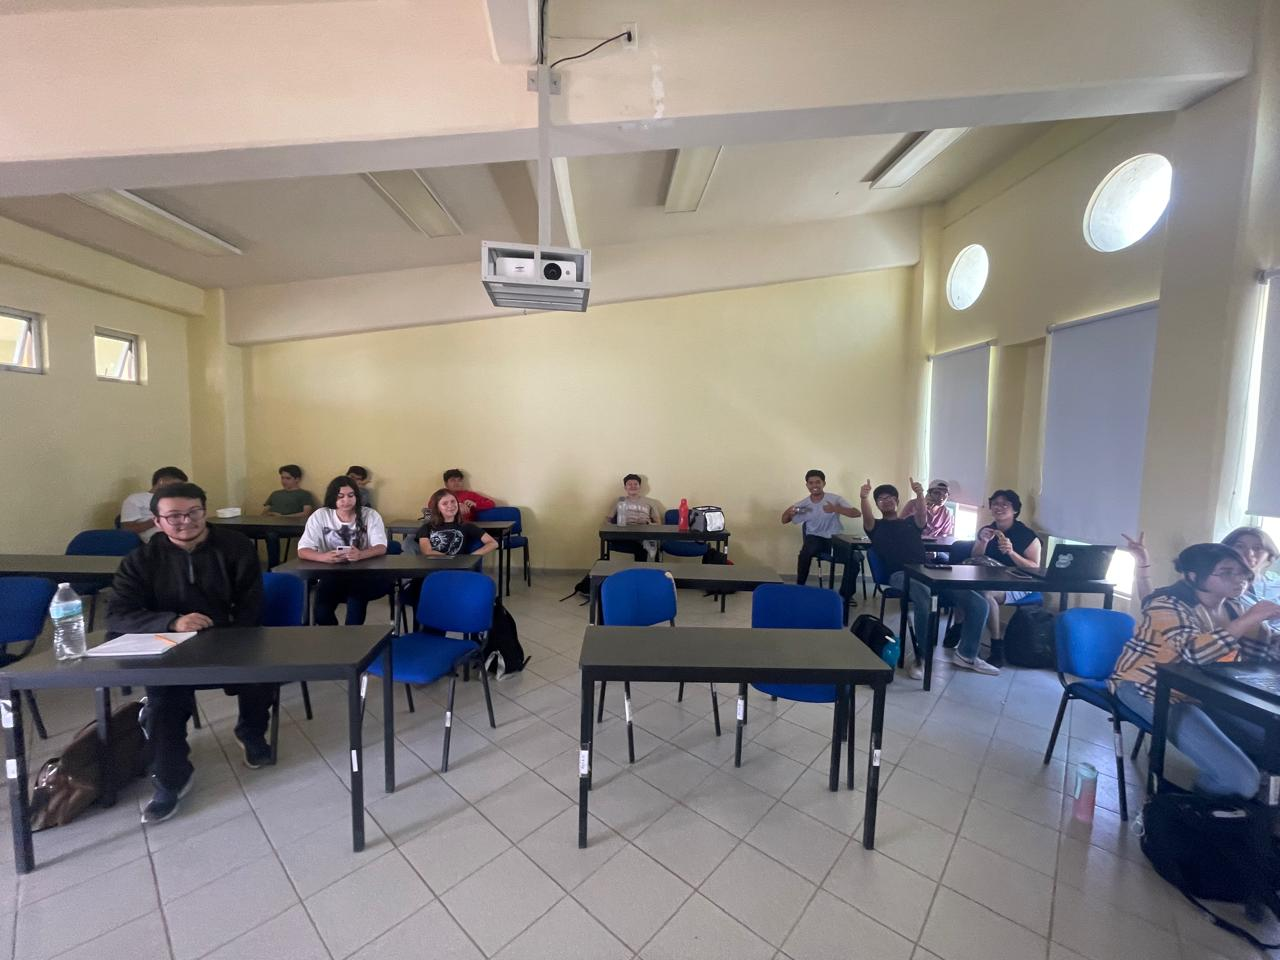
\includegraphics[width=0.7\textwidth]{./assets/img/imagen3DH.jpeg}
\end{figure}

\begin{figure}
    \caption{El día 7 de mayo de 2024 se hizo incapi\'e en la r\'ubrica de evaluaci\'on del proyecto final de la materia "Desarrollo Humano II". Grupo 31, 2024.\label{fig:No.4}}
    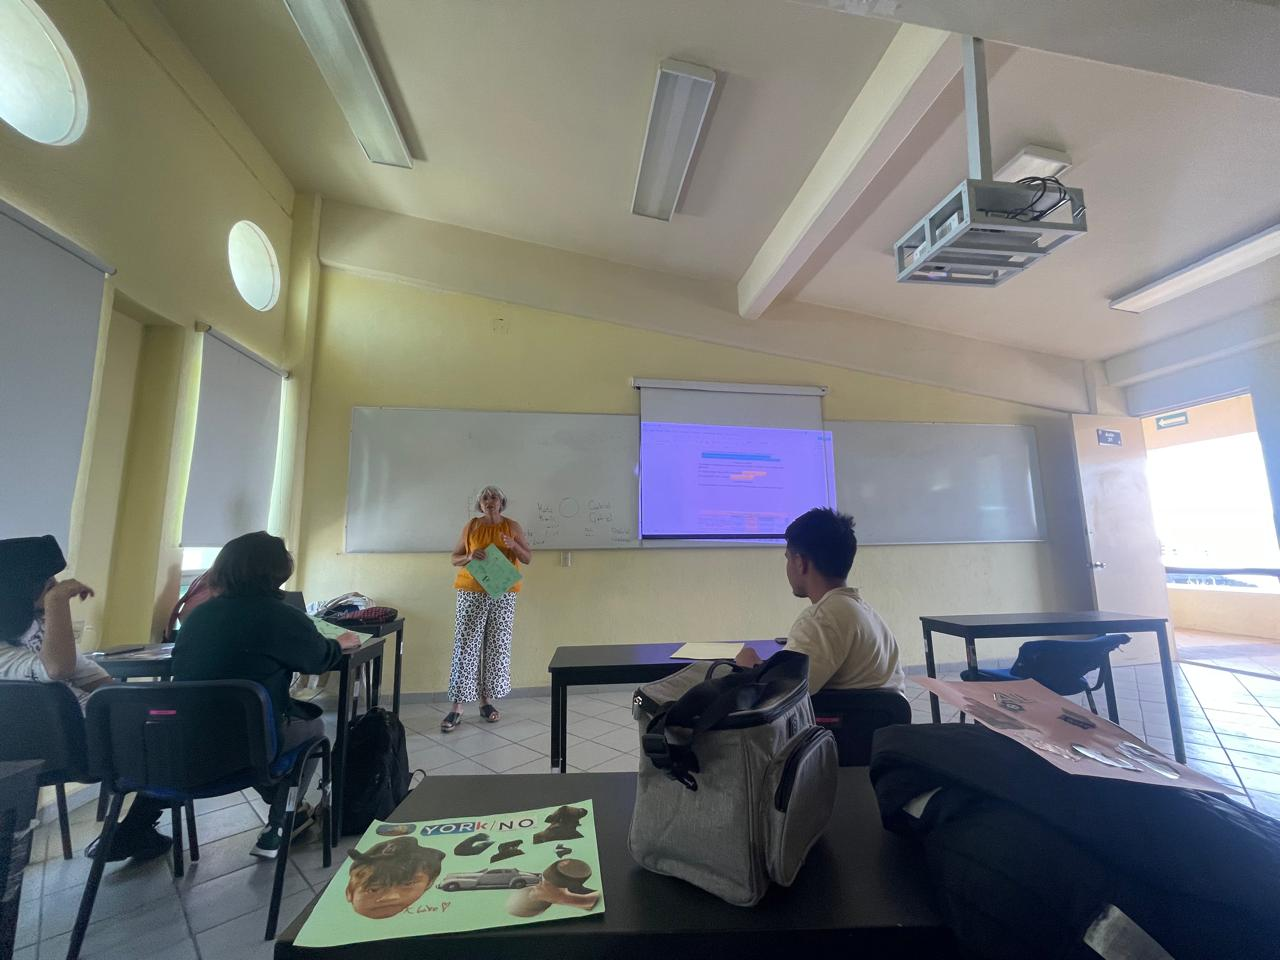
\includegraphics[width=0.7\textwidth]{./assets/img/imagen4DH.jpeg}
\end{figure}

\begin{figure}
    \caption{El d\'ia 14 de mayo de 2024 se realiz\'o una actividad recreativa haciendo uso de la m\'imica con la inteligencia visual-espacial. Grupo 31,2024.\label{fig:No.5}}
    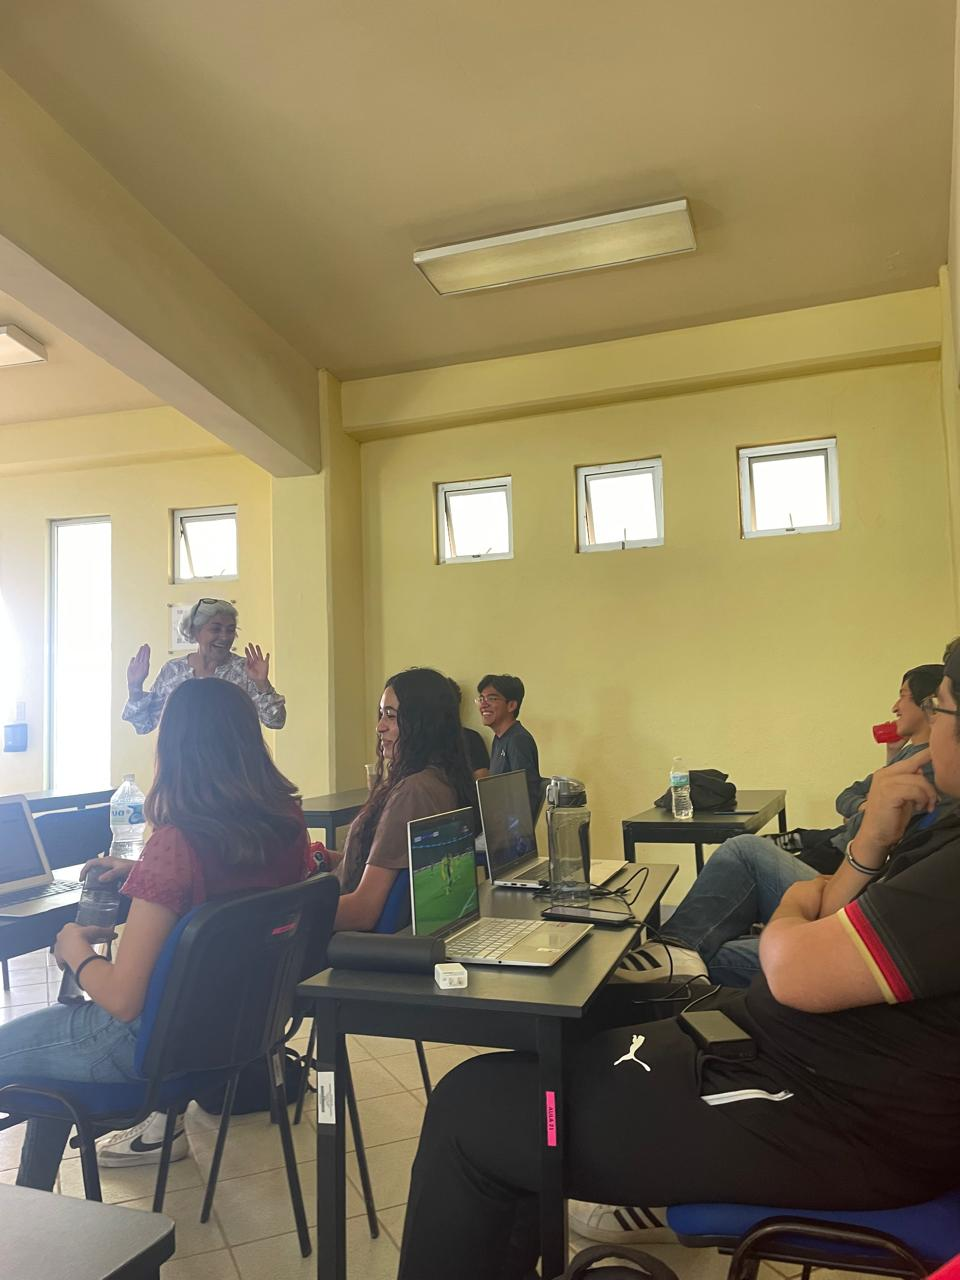
\includegraphics[width=0.7\textwidth]{./assets/img/imagen5DH.jpeg}
\end{figure}

\begin{figure}
    \caption{El d\'ia 16 de mayo de 2024 se llev\'o a cabo el examen del 3er Parcial de la materia "Desarrollo Humano II". Grupo 31, 2024.\label{fig:No.6}}
    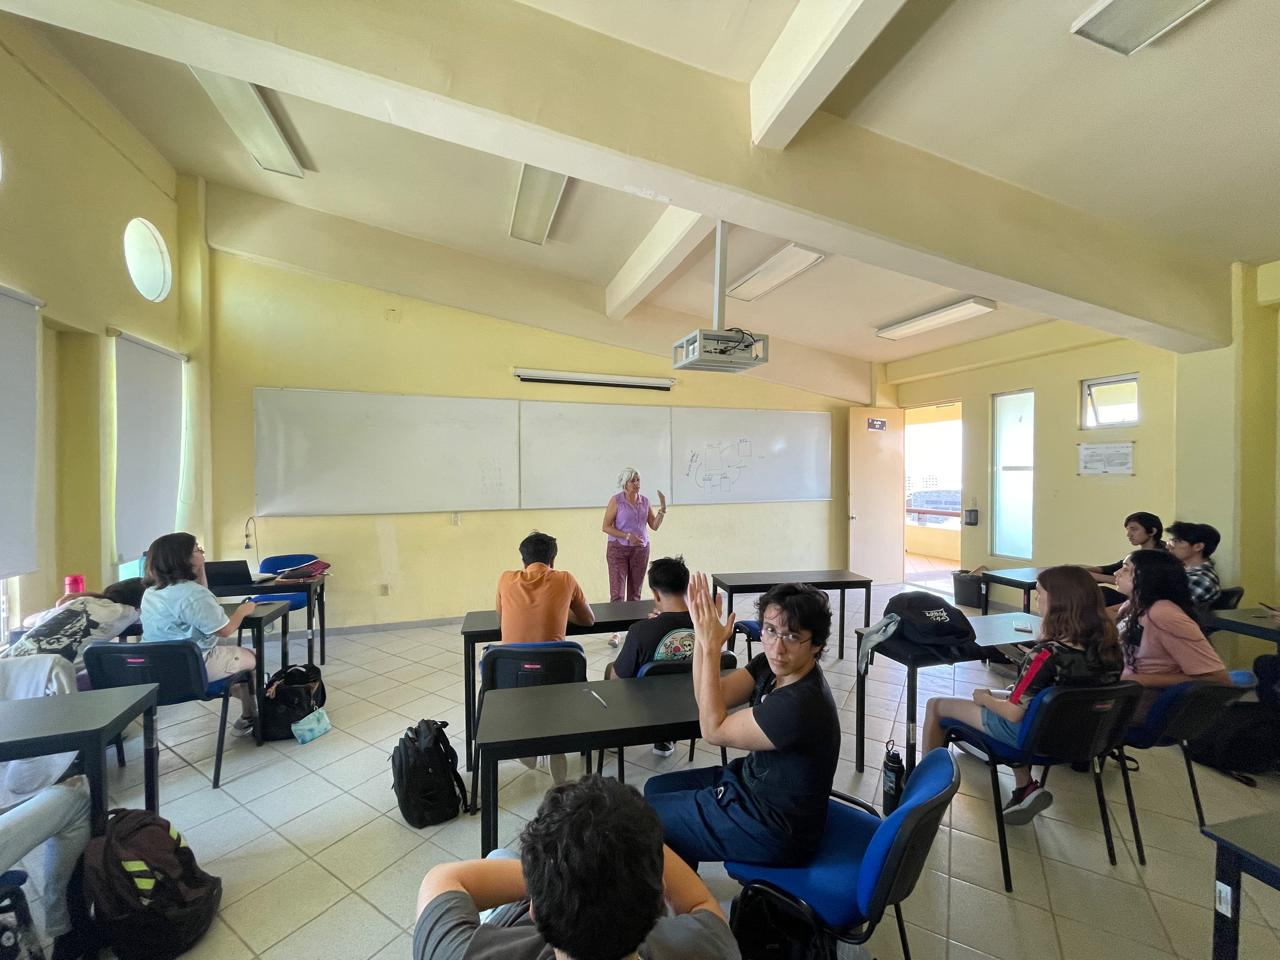
\includegraphics[width=0.7\textwidth]{./assets/img/imagen6DH.jpeg}
\end{figure}

\end{appendix}
\printbibliography
\end{document}
